%%%%%%%%%%%%%%%%%%%%%%%%%%%%%%%%%%%%%%%%%%%%%%%%%%%%%%%%%%%%%%%%%%%%%
% Presentation template												%
% 																	%	
% Radmir Gesler														%
% 10.11.18															%
% By using of BHT template											%
%																	%
%%%%%%%%%%%%%%%%%%%%%%%%%%%%%%%%%%%%%%%%%%%%%%%%%%%%%%%%%%%%%%%%%%%%% 
%																	%
% Document settings, packages.										%
%																	%
%%%%%%%%%%%%%%%%%%%%%%%%%%%%%%%%%%%%%%%%%%%%%%%%%%%%%%%%%%%%%%%%%%%%%
\documentclass[10pt]{beamer}
\usetheme{BHT}

\usepackage{helvet}
\usepackage[ngerman]{babel}
\usepackage[latin1]{inputenc}
\usepackage{graphicx}
\usepackage{longtable, tabularx}
\usepackage{multicol, multirow}
\usepackage{listings, pifont,  verbatim}

\usepackage{subfig} 

\usepackage{ifthen, xspace}
\usepackage{colortbl}
%\usepackage{mathptmx}
\usepackage{tikz}




\newtheorem{Bemerkung}{Bemerkung}
%\newtheorem{Definition}{Definition}

\newcommand{\uproman}[1]{\uppercase\expandafter{\romannumeral#1}}
\newcommand{\lowroman}[1]{\romannumeral#1\relax}

\newcommand{\captionstring}[1]{\noexpand\noexpand\noexpand\string\string#1}



%\usefonttheme{professionalfonts}
%\usepackage{unicode-math}



\newcommand{\R}{ \mathbb{R} }
\newcommand{\N}{ \mathbb{N} }



%%%%%%%%%%%%%%%%%%%%%%%%%%%%%%%%%%%%%%%%%%%%%%%%%%%%%%%%%%%%%%%%%%%%% 
%																	%
% Project settings													%
%																	%
%%%%%%%%%%%%%%%%%%%%%%%%%%%%%%%%%%%%%%%%%%%%%%%%%%%%%%%%%%%%%%%%%%%%%
\setbeamercovered{transparent}
\graphicspath{{pictures/}}

\title[]%[Rekonstruktionsverfahren f�r Computertomographie-Bilddaten]
      {Rekonstruktionsverfahren f�r Computertomographie-Bilddaten}

\date{\today}
\institute{Pr�sentation der Bachelorarbeit}
\author{Radmir Gesler}


%\usefonttheme{serif}
\usefonttheme[onlymath]{serif}

%%%%%%%%%%%%%%%%%%%%%%%%%%%%%%%%%%%%%%%%%%%%%%%%%%%%%%%%%%%%%%%%%%%%
\begin{document}
	
%	\newtheorem{Definition}{Definition}
	

\frame{\titlepage}
\setbeamerfont{frametitle}{size=\small}

%%%%%%%%%%%%%%%%%%%%%%%%%%%%%%%%%%%%%%%%%%%%%%%%%%%%%%%%%%%%%%%%%%%%
%% Inhalt
%%

%\setcounter{part}{1}
%\setcounter{part}{-1}
%\part{Praktische T�tigkeit bei GFaI e.V.}

%\frame{\partpage}

\frame{\frametitle{Ablauf der Pr�sentation}
	\begin{enumerate}
		\item[1] Computertomographie, das Prinzip und Modell \pause
		\item[2] Computertomographie als inverses Problem \pause
		\item[3] Rekonstruktionsverfahren
		\begin{itemize}
			\item[3.1] Ungefilterte R�ckprojektion
			\item[3.2] Gefilterte R�ckprojektion
			\item[3.3] Iterative Rekonstruktion nach Kaczmarz
			\item[3.4] Rekonstruktion durch Singul�rwertzerlegung
		\end{itemize}
	\end{enumerate}
} 

\frame{\frametitle{1. Computertomographie: das Prinzip} 
	\centering
	\begin{tikzpicture}
		\draw[dashed,color=gray][rotate=90] (0,0) arc (-90:90:0.5 and 1.5);% top half of the bottom ellipse
		
		\draw[semithick][rotate=90] (4,1.5) arc (0:360:0.5 and 1.5);
		\draw[very thin, ->][rotate=95] (2.3,-2) arc (240:340:1.6 and 6);
		
		\fill[nearly transparent][rotate=90] (2.25,1.5) arc (0:360:0.5 and 1.5); % middle ellipse
		
		% inner lines
		\draw[dashed,color=gray] [rotate=90] (0,1.2) -- (3.5,1.2);% left line of inner small ellipse 
		\draw[dashed,color=gray] [rotate=90] (0,0.6) -- (3.5,0.6);% right line of the inner small ellipse
		
		\draw[dashed,color=gray] [rotate=90] (3.5, 2.35) -- (0, 2.35);% right line of the inner big ellipse
		\draw[dashed,color=gray] [rotate=90] (3.5, 1.45) -- (0, 1.45);% left line of the inner big ellipse
		
		% inner top ellipses
		\draw[semithick] [rotate=90] (3.5, .9) ellipse (0.1 and .3); % top small inner ellipse
		\draw[semithick] [rotate=90] (3.5, 1.9) ellipse (0.2 and .45); % top big inner ellipse
		
		% inner middle ellipses
		\fill[nearly opaque,color=orange] [rotate=90] (1.8, .9) ellipse (0.1 and .3);% middle small inner ellipse
		\fill[nearly opaque,color=orange] [rotate=90] (1.8, 1.9) ellipse (0.2 and .45); % middel big inner ellipse
		\draw[dashed,color=gray] [rotate=90] (1.8, .9) ellipse (0.1 and .3);% middle small inner ellipse
		\draw[dashed,color=gray] [rotate=90] (1.8, 1.9) ellipse (0.2 and .45); % middel big inner ellipse
		
		
		% inner bottom ellipses
		\draw[dashed,color=gray] [rotate=90] (0, .9) ellipse (0.1 and .3); % bottom small inner ellipse
		\draw[dashed,color=gray] [rotate=90] (0, 1.9) ellipse (0.2 and .45); % bottom big innerellipse
		
		\draw[color=orange][rotate=90] (2.25,1.5) arc (0:360:0.5 and 1.5); % middle ellipse
		
		%sids lines
		\draw[semithick] [rotate=90] (0,0) -- (3.5,0);% right line
		\draw[semithick] [rotate=90] (0,3) -- (3.5,3);% left line
		
		% R�ntgenr�hre
		\draw [semithick] [rotate=30, xshift=0.cm, yshift=-1.0cm](0.2,0) -- (2.6,0); % R�ntgenr�hre
		\draw  (1.5,-1.4) node [rotate=30, xshift=1.cm, yshift=0.5cm] { R�ntgenr�hre};
		
		\draw [semithick] [rotate=30, xshift=-3.5cm, yshift=5.3cm](0.2,0) -- (2.5,0); % Detektorachse
		\draw  (1.5,-1.4) node [rotate=30, xshift=-3.3cm, yshift=8.3cm] {Detektor};
		
		\draw [dashed, semithick, <-, blue] [rotate=150, , xshift=1.cm, yshift=0.1cm](5,0) -- (-2,0);
		\draw [dashed, semithick, <-, blue] [rotate=150, , xshift=0.8cm, yshift=-0.34cm](5,0) -- (-2,0);
		\draw [dashed, semithick, <-, blue] [rotate=150, , xshift=0.55cm, yshift=-0.75cm](5,0) -- (-2,0);
		\draw [dashed, semithick, <-, blue] [rotate=150, , xshift=0.3cm, yshift=-1.2cm](5,0) -- (-2,0);
		\draw [dashed, semithick, <-, blue] [rotate=150, , xshift=3.cm, yshift=-1.63cm](2,0) -- (-5,0);
		
		\fill[gray] [rotate=30, yshift=5.4cm, xshift=-3cm] (-0.3,0) .. controls (0.1,0.6) and (1,0.4) .. (1.9,0);
		\fill[gray] [rotate=30, yshift=5.4cm, xshift=-3cm] (0.3,0) .. controls (0,0.8)  .. (1,0);
		\fill[gray] [rotate=30, yshift=5.4cm, xshift=-3cm] (1,0) .. controls (0.7,0.6)  .. (1.4,0);
		
		\draw[semithick] [rotate=90] (0,0) arc (270:90:0.5 and 1.5);% bottom half of the bottom ellipse		
	\end{tikzpicture}
} 

\frame{\frametitle{1. Computertomographie: das Modell}
	
	\centering
	\begin{tikzpicture}	
		\fill[nearly transparent, color=gray] (0.9,0) circle (1.8cm);
		
		\fill[lightgray] (0.9,0) ellipse (1.6cm and 1.2cm);	
		
		\draw[orange] (0.9,0) ellipse (1.6cm and 1.2cm);
		
		\draw [gray] [->](-1.3,0) -- (3,0); % x-Achse
		\draw [gray] (3, 0) node [right] {$\displaystyle x$};
		
		\draw [gray] [->](0.9,-2) -- (0.9,2); % y-Achse
		\draw [gray] (0.9, 2.2) node {$y$};
		
		\draw[gray](0.9, 0.3) node [left] {$\mbox{supp}f$};
		
		\draw[->] (0.9,0) -- (2, 0.7);
		\draw(1.2, 0.5)  node [right] {$s$};
		
		\draw [rotate=30, xshift=2.1cm, dashed, ->] [blue] (0,-3) -- (0,2.3); % strahl
		\draw [blue] (0.55, 2.5)  node {$L$};
		
		\draw(2,0) arc [start angle=0, end angle=35, radius=1cm];
		\draw(1.5, 0.2) node [right] {$\theta$};
		
		\draw [gray] (-0.8, -1.5) node [right] {$\Omega$};
		
		\draw(3.9, 1.3) node {$I(L_0 + \Delta L)$};
		\fill[gray](2.25, 0.3) circle [radius=0.06];
		\draw[-,thin,gray](2.25, 0.3) -- (3, 1.1);
		
		\draw(3.9, -0.9) node {$I(L_0)$};
		\fill[gray](2.65, -0.4) circle [radius=0.06];
		\draw[-,thin,gray](2.65, -0.4) -- (3.4, -0.8);
	\end{tikzpicture}
	\begin{equation*}
		I(L_0 + \Delta L) - I(L_0) = - f(L)\parallel \Delta L \parallel I(L_0).
	\end{equation*}	
}

\frame{\frametitle{1. Computertomographie: das Modell}
	\begin{Definition}
		Sei nun $f:\Omega \subseteq \R^2 \rightarrow \R$ eine integrierbare Funktion, dann ist ihre Radon Transformation durch
		\begin{equation}
			\mathcal{R}f(s,\theta) := \int\limits_{-\gamma(s)}^{\gamma(s)} f(L(s,\theta,t)) \mbox{d}t
			\label{equa:1}
		\end{equation}
		definiert. Hier ist $\Omega = \{ (x,y) \in \R^2 \ | \ x^2 + y^2 \leq 1 \}$.
	\end{Definition}

	\begin{equation} \pause
		\begin{matrix}
		L(s, \theta, t) & = & s\begin{pmatrix} \cos(\theta) \\ \sin(\theta) \end{pmatrix} & + & t\begin{pmatrix} -\sin(\theta) \\ \cos(\theta)  \end{pmatrix} \\ \\
		& = & s\omega(\theta) & + & t\omega^{\perp}(\theta)
		\end{matrix} \ , \ \ s, t \in \R; \ \theta \in [0,\pi].
		\label{equa:2}
	\end{equation}

	\begin{equation} \pause
		\gamma(s) = \left\{ \begin{matrix}
		\sqrt{1 - s^2} & : & |s| \leq 1 \\ 
		0 & : & \mbox{sonst}
		\end{matrix}.
		\right.
		\label{equa:3}
	\end{equation}
}

\frame{\frametitle{1. Computertomographie: das Modell}
	Im Folgenden betrachten wir die Radon-Transformation als $\mathcal{R} : L^2(\Omega) \rightarrow L^2(Z)$. \vspace{20pt} \\ \pause
	
	Die Radon Transformation ist:
	\begin{itemize}
		\item[1.] Linear, also $\mathcal{R}( \alpha f + \beta g) = \alpha \mathcal{R} f +  \beta \mathcal{R}sg$. \pause
		\item[2.] $\mathcal{R}$ ist beschr�nkt $\Vert \mathcal{R} f(s,\theta) \Vert_{L^2(Z)}^2 \leq 2\pi \Vert f \Vert_{L^2(\Omega)}^2$, somit auch stetig. \pause
		\item[3.] $\mathcal{R}$ hat einen adjungierten Operator $\mathcal{R}^*:L^2(Z) \rightarrow L^2(\Omega)$ 
		\begin{equation}
			\mathcal{R^*} g(x) = \int\limits_{0}^{\pi} \ g(x^{T}\omega(\theta),\theta) \mbox{d}\theta.
			\label{equa:5}
		\end{equation} \pause
		\item[4.] $\mathcal{R}$ ist kompakt, somit ist auch $\mathcal{R^*}$ kompakt (nach Satz von Schauder).
	\end{itemize}
}

\frame{\frametitle{1. Computertomographie: das Modell}
	Anhand der obigen Eigenschaften von $\mathcal{R}$ ist es m�glich die Singul�rwertzerlegung f�r $\mathcal{R}:L^2(\Omega) \rightarrow L^2(Z)$ anzugeben (\textit{Spektralsatz f�r selbstadjungierte kompakte Operatoren}). 
	\begin{equation}
		\mathcal{R}f = \sum\limits_{j = 1}^{\infty} \sigma_j \langle f, v_j\rangle_{L^2(\Omega)} u_j.
		\label{equa:1.32}
	\end{equation}\pause
	Hier bezeichnen:
	\begin{itemize}
		\item $\{v_j\}_{j \in \N} \in L^2(\Omega)$ das Orthonormalsystem (ONS) von $\mbox{Kern}(\mathcal{R})^\perp$. \pause
		\item $\sigma_j := \sqrt{\lambda_j}$, wobei $\{\lambda_j\}_{j \in \N}$ eine positive absteigende Folge der Eigenwerten von $\mathcal{RR^*}$, die entweder abbricht oder gegen Null geht.\pause
		\item $u_j := \sigma^{-1}\mathcal{R}v_j$, sodass $\{u_j\} \in L^2(Z)$ das ONS von $\overline{\mbox{Bild}(\mathcal{R})}$ ist.
	\end{itemize}
}


\frame{\frametitle{2. Computertomographie als inverses Problem}
	�bertragung auf das Rekonstruktionsproblem aus den CT-Bilddaten  
	\begin{center}
		\begin{tikzpicture}[xshift=-100, scale=0.75]
		
		\draw [gray] (0, 0.5) [rotate=0, xshift=0, yshift=0] node {unbekannte};
		\draw [gray] (0,0)  [rotate=0, xshift=0, yshift=0] node {Dichteverteilung};
		\draw [gray] (0,-0.5)  [rotate=0, xshift=0, yshift=0] node {$f$};
		\fill[nearly transparent, color=gray] (0,0) circle (1.8cm);
		
		\draw [gray] (3.1, 0) [rotate=0, xshift=0, yshift=70] node {invers};
		\draw[<-, gray] [rotate=0, xshift=90, yshift=50] (-2,0) to[out=15, in=165] (2,0);
		
		\draw [gray] (3.1, 0) [rotate=0, xshift=0, yshift=-40] node {direkt};
		\draw[->, gray] [rotate=0, xshift=90, yshift=-50] (-2,0) to[out=-15, in=195] (2,0);	
		
		\draw [gray] (6.3, 0) [rotate=0, xshift=0, yshift=0] node {Projektionen $p$};
		\fill[nearly transparent, color=gray] (6.3,0) circle (1.8cm);
		\end{tikzpicture}
	\end{center}
	Das hei�t, man sucht nach einer zu $\mathcal{R}$ inversen Abbildung, sodass aus den Projektionsdaten die unbekannte Dichteverteilung $f$ berechnet werden kann.
}

\frame{\frametitle{2. Computertomographie als inverses Problem}
	M�gliche Invertierung des Operators $\mathcal{R}$ kann aus der Gleichung \ref{equa:5} hergeleitet werden:
	\begin{equation}
		\mathcal{R^+}g = \sum\limits_{j = 1}^{\infty} \sigma_j^{-1} \langle g, u_j\rangle_{L^2(Z)} v_j.
		\label{equa:6}
	\end{equation} \pause
	Problem:\\
	\begin{center}
		%$\sigma_j \xrightarrow[{j \rightarrow \infty}]{} 0 \ \ \ \ \mbox{also} \ \ \ \ 
		$\sigma_j^{-1} \xrightarrow[{j \rightarrow \infty}]{} \infty$\\
		Was zu einer Oszillation in der L�sung f�hren kann.
	\end{center} \pause
	Ziel: 
	\begin{center}
		Die Oszillation zu d�mpfen, was im allgemeinen als \textbf{Regularisierung} bezeichnet wird.
	\end{center}	
}

\frame{\frametitle{3. Rekonstruktionsverfahren}
	\textbf{Bedingung:} die Rekonstruktionsverfahren werden f�r parallele Strahlengeometrie betrachtet.	
	\begin{center}
		\includegraphics[width=0.49\textwidth]{phantom.eps}
		\includegraphics[width=0.49\textwidth]{rt_phantom.eps} 
	\end{center}
	\begin{equation}
		\mathcal{R}f(s,\theta) := \int\limits_{-\gamma(s)}^{\gamma(s)} f(L(s,\theta,t)) \mbox{d}t
	\end{equation}
}

\frame{\frametitle{3. Rekonstruktionsverfahren: Ungefilterte R�ckprojektion}
	Die ungefilterte R�ckprojektion ist genau der adjungierte Operator zu $\mathcal{R}$
	\begin{equation}
		\begin{split}
			\mathcal{R^*} g(x) & = \int\limits_{0}^{\pi} \ g(x^{T}\omega(\theta),\theta) \mbox{d}\theta \\
			\mathcal{R^*} g(x_0) & = f(x)*h(x) = f(x)*\frac{1}{|x - x_0|}
		\end{split}
	\end{equation}
	\begin{center}
		\includegraphics[width=0.5\textwidth]{backProjection.eps}
	\end{center}
}

\frame{\frametitle{3. Rekonstruktionsverfahren: Gefilterte R�ckprojektion}
	Die Regularisierung erfolgt durch verschiedene Filterfunktionen $h_{\xi}(q)$.
	\begin{equation}
		f(x) = \int \limits_{0}^{\pi} \left( \int \limits_{-1}^{1} \left( \ P(q, \theta)h_{\xi}(q) \ \right) e^{2\pi i qx^T\omega(\theta)} \ \mbox{d}q \right) \mbox{d}\theta
	\end{equation}
	Wobei hier $P(q, \theta)$ die Fouriertransformierte der Projektion ist. 
	\begin{center}
		\includegraphics[width=0.49\textwidth]{rampFilter.eps}
		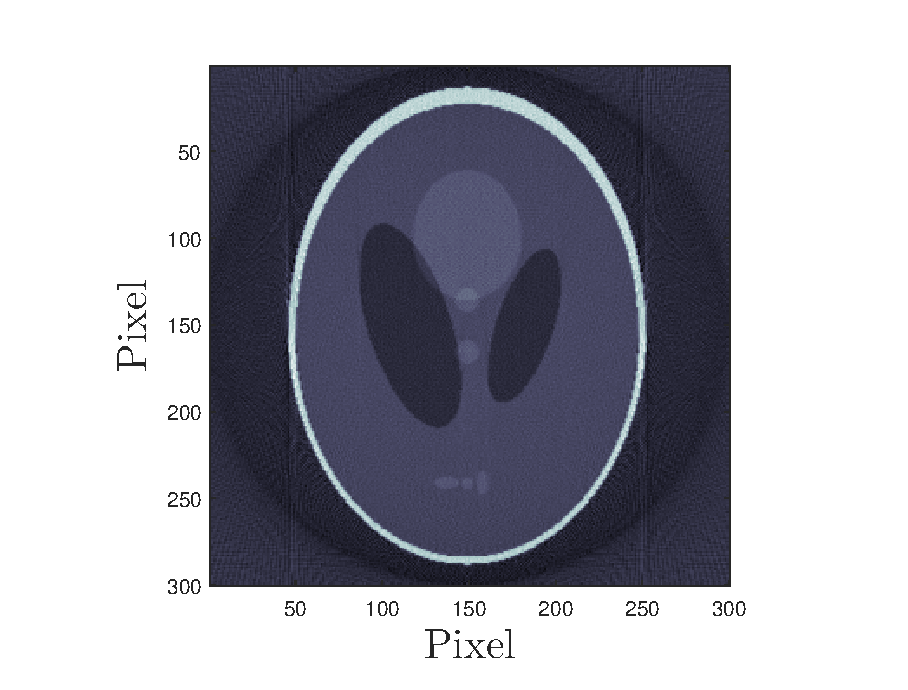
\includegraphics[width=0.49\textwidth]{rampFiltered.eps} 
	\end{center}
}

\frame{\frametitle{3. Rekonstruktionsverfahren: Iterative Rekonstruktion}
	Hier fasst man den Operator $\mathcal{R}$ als eine lineare Abbildung
	\begin{equation}
		\mathcal{R}f = Af = p
	\end{equation}
	auf. Die Anzahl der Zeilen von $A$ ist gleich der Anzahl der Projektionen und die Anzahl der Spalten gleicht der Zahl der Diskretisierungsstellen zum Quadrat.\\ \pause 
	So l�sst sich (10) in ein Gleichungssystem umschreiben
	\begin{equation}
	\begin{split}
	a_{11}f_1 + \ \ \dots \ \ + a_{1m}f_m & = p_1 \\
	& \ \ \vdots\\
	a_{j1}f_1 + \ \ \dots \ \ + a_{jm}f_m & = p_j \\
	& \ \ \vdots\\
	a_{n1}f_1 + \ \ \dots \ \ + a_{nm}f_m & = p_n.
	\end{split}
	\label{equa:3.24}
	\end{equation}	 
}

\frame{\frametitle{3. Rekonstruktionsverfahren: Iterative Rekonstruktion}
	\begin{figure}[H]
		\begin{tikzpicture}[scale=0.5]
			\draw [gray] [->](-2,0) -- (3,0); % x-Achse
			\draw [gray] (3, 0) node [right] {$x_1$};
			
			\draw [gray] [->](0,-2) -- (0,3); % y-Achse
			\draw [gray] (0, 3.2) node {$x_2$};
			
			\draw [rotate=-40, xshift=1cm, yshift=1cm] [blue] (3,0) -- (-4,0); % blue ray	
			\draw [gray, xshift=3.7cm, yshift=-1.3cm] (0,0) node {$H_2$};
			
			\draw [rotate=10, xshift=1cm, yshift=1cm] [blue] (4,0) -- (-3,0); % blue ray
			\draw [gray, rotate=10, xshift=5cm, yshift=1.3cm] (0,0) node {$H_1$};
			
			\draw [rotate=100, xshift=1cm, yshift=-3cm, dashed] [green] (0,0) -- (1.5,0); % green from strat
			\fill[color=gray, xshift=1cm, yshift=3cm] (1.5,0) circle (0.05cm); % f point
			\draw [color=black, xshift=1cm, yshift=3cm] (1.5,0.3) node {$f_0$};
			
			\draw [rotate=50, xshift=1cm, yshift=-1.2cm, dashed] [green] (0,0) -- (2,0); % green from strat
			\fill[color=gray,rotate=50, xshift=1.4cm, yshift=-1.2cm] (1.5,0) circle (0.05cm); % f 1 point
			\draw [color=black,xshift=1.4cm, yshift=1.2cm] (1.5,0) node {$f_1$};
			
			\draw [rotate=100, xshift=-0.3cm, yshift=-1.5cm, dashed] [green] (0,0) -- (1.3,0); % green from strat	
			\fill[color=gray,rotate=50, xshift=1cm, yshift=-1.2cm] (0,0) circle (0.05cm); % f 2 point
			%\draw [color=black, xshift=1.45cm, yshift=-0.2cm] (0,0) node {$f_2$};
			
			\draw [rotate=100, xshift=-0.3cm, yshift=-1.5cm, dashed] [green] (0,0) -- (1.3,0); % green from strat	
			\fill[color=gray,rotate=100, xshift=-0.3cm, yshift=-1.5cm] (1.3,0) circle (0.05cm); % f 3 point
			\draw [color=black, xshift=0.1cm, yshift=1.5cm] (1.3,0) node {$f_t$};
			
			\draw [rotate=50, xshift=0.3cm, yshift=-0.2cm, dashed] [green] (0.7,0) -- (1.3,0); % green from strat		
			\fill[color=gray, rotate=50, xshift=0.3cm, yshift=-0.2cm] (0.7,0) circle (0.05cm); % f 4 point
			%\draw [color=black, xshift=0.1cm, yshift=0.3cm] (0.7,0) node {$f_4$};
			
			\draw [rotate=100, xshift=-0.2cm, yshift=-0.9cm, dashed] [green] (0.7,0) -- (1.3,0); % green from strat	
			\fill[color=gray, rotate=100, xshift=-0.2cm, yshift=-0.9cm] (1.2,0) circle (0.05cm); % f point
			
			\fill[color=gray, xshift=0.3cm, yshift=1.06cm] (0,0) circle (0.05cm); % f point
			\draw [color=black, xshift=0.3cm, yshift=1.3cm] (0,0) node {$f$};
		\end{tikzpicture}
	\end{figure}	 
	\begin{Definition}[Randomisierter Kaczmarz-Algorithmus]
		Sei $Af = p$ ein konsistentes, lineares Gleichungssystem. Sei $f_0 \in \R^m$ ein beliebiger Startwert. F�r $t = 0, 1, 2, ...$ ist der Randomisierte Kaczmarz-Algorithmus definiert als
		\begin{equation}
		f_{t+1} = f_t + \frac{p_j - \langle a_j, f_t \rangle}{\parallel a_j \parallel_{2}^{2}}a_j,
		\label{equa:3.25}
		\end{equation}
		wobei $a_j$ die $j$-te Zeile von $A$ ist und $p_j$ die dazugeh�rige Projektion. $j$ wird zuf�llig ausgew�hlt.
		\label{def:5}	
	\end{Definition} 
}

\frame{\frametitle{3. Rekonstruktionsverfahren: Iterative Rekonstruktion}
	Die Regularisierung erfolgt durch die Anzahl der Iterationen, hier mit 3 Iterationen.
	\begin{center}
		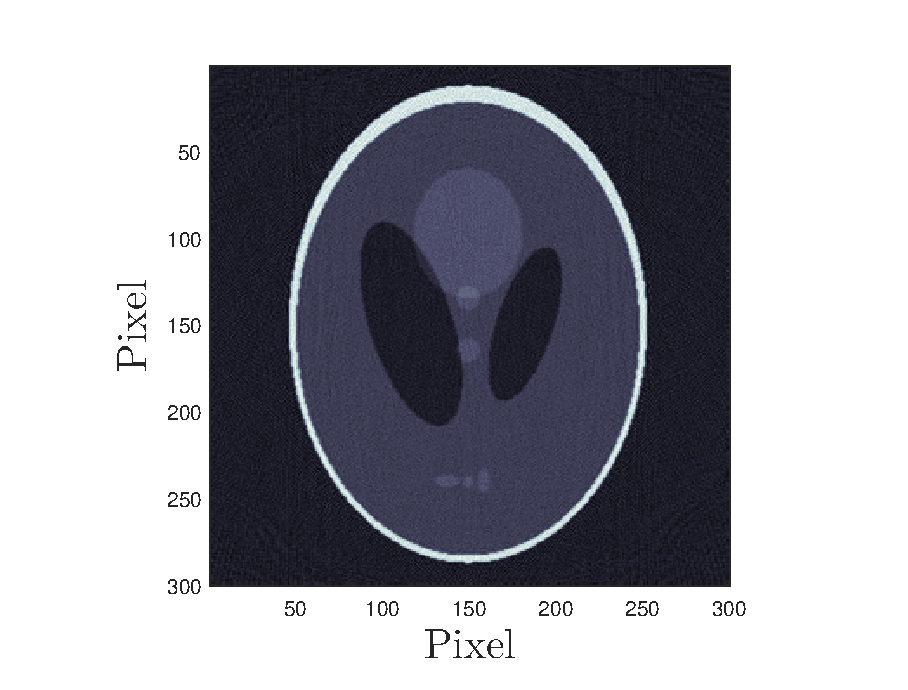
\includegraphics[width=0.5\textwidth]{iter.eps}
	\end{center}
}

\frame{\frametitle{3. Rekonstruktionsverfahren: Rekonstruktion durch SWZ}
	\begin{equation}
		\mathcal{R}f = Af = (U\Sigma V^*)f = p
	\end{equation}
	Invertierung von (13) f�hrt zum Ergebnis
	\begin{equation}
		f = (V\Sigma^+ U^*)p
	\end{equation}
	Rechenergebnisse mit der Tikhonov-Regilarisierung $[\Sigma^+]_{ii} = \frac{\sigma_j}{\lambda^2+\sigma_j^2}$.
	\begin{figure}[!h]
		\centering
		\includegraphics[width=0.85\textwidth]{svdRedANDnotReg.eps}
	\end{figure}
}

\frame{\frametitle{3. Rekonstruktionsverfahren: Gegen�berstellung der Verfahren}
	\begin{figure}[!h]
		\centering
		\includegraphics[width=0.9\textwidth]{ALL.eps}
	\end{figure}
}


\frame{\frametitle{Abschluss}
	\centering
	Vielen Dank f�r Ihre Aufmerksamkeit.\\
	F�r Fragen und Anregungen stehe ich Ihnen gerne zur Verf�gung.
}


\end{document}
%%%%%%%%%%%%%%%%%%%%%%%%%%%%%%%%%%%%%%%%%%%%%%%%%%%%%%%%%%%%%%%%%%%%